
\begin{figure}[h!]
	%\begin{wrapfigure}[20]{r}{7cm}\footnotesize
	%\vspace{-1em}
	~~~~~~~~~~~~~~~~~~~~~~\footnotesize
	\begin{center}
		\begin{tikzpicture}[node distance=.7cm,minimum height=.5cm]
			% nodes
			\node[draw] (mps) 			   {MPS};
			\node[draw, right =3cm of mps, yshift=-1.5cm] (limdd) {\limdd};
			%		\node[draw, above =of limdd, yshift=1.5cm] (tn) {TN};
			\node[draw, right =3cm of limdd, yshift=1.5cm] (rbm) {RBM};
			%		\node[draw, below =2cm of rbm, xshift=0.4cm,text width=1.3cm, align=center] (ss) {Stabilizer States};
			\node[draw, below = 1cm of limdd] (qmdd) {\qmdd};
			\node[draw, below = .6cm of qmdd] (add) {ADD};
			\node[draw, below = .6cm of add, xshift= 0cm] (statevec) {State Vector};
			
			% edges
			\draw[\bigarrowhead, dashed,  bend left=20] (limdd.west) \limddToMpsLabel (mps.south);
			\draw[\bigarrowhead, dashed,  bend left=20] (mps.south east) \mpsToLimddLabel (limdd.north west);
			\draw[\bigarrowhead, dashed, bend left=5] (rbm.west) \rbmToMpsLabel (mps.east);
			\draw[\bigarrowhead, dashed,  bend left=20] (mps.north east) to node[midway,fill=white,draw,solid] {?} (rbm.north west);
			\draw[\bigarrowhead, dashed,  bend right=20] (limdd.east) to node[midway,fill=white,draw,solid] {?} (rbm.south);
%			\draw[\bigarrowhead, bend right=30] (statevec) \statevecToAddLabel (add);
			\draw[\bigarrowhead, dashed, bend right=30] (add) \addToStatevecLabel(statevec);
%			\draw[\bigarrowhead, bend right=20] (add) \addToQmddLabel (qmdd);
			\draw[\bigarrowhead, dashed, bend right=30] (qmdd) \qmddToAddLabel (add);
			\draw[\bigarrowhead, dashed, bend right=30] (rbm.south west) \rbmToLimddLabel (limdd.north east);
			\draw[\bigarrowhead, dashed, bend right=30] (limdd) \limddToQmddLabel (qmdd);
%			\draw[\bigarrowhead, bend left=50] (qmdd.west) \qmddToMpsLabel (mps.south west);
			%		\draw[\bigarrowhead, bend left=20] (mps) to (tn);
			%		\draw[\bigarrowhead, bend right=20] (rbm) to (tn);
			%		\draw[\bigarrowhead] (ss) to (limdd);
			%		\draw[\bigarrowhead] (ss) to (rbm.south east);
%			\draw[\bigarrowhead, bend right=30] (qmdd) \qmddToLimddLabel (limdd);
			%		\draw[\bigarrowhead, dashed] (qmdd.east) to (ss.west);
		\end{tikzpicture}
		%    \vspace{-1em}
		%    \vspace{-3em}
		%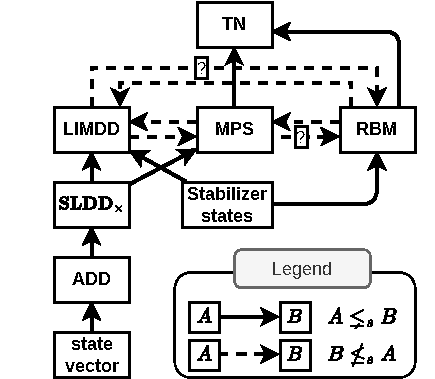
\includegraphics[width=0.4\textwidth]{pics/succinctness-relations.pdf}
		\caption{Separations between various classical data structures for representing quantum states.
%			A solid arrow $A\to B$ indicates that one data structure is strictly more succinct than another ($B\strictlymoresuccinctthan A$). 
			A dotted arrow $A\to B$ indicates a separation ($A\notmoresuccinctthan B$), i.e., there is some state that $A$ can represent, which $B$ cannot efficiently represent.
			%, e.g., the dotted arrow from RBM to MPS indicates that RBMs can efficiently represent some states for which MPS requires exponential size (in this case, some stabilizer states, among others).
			A question mark means the relation is unknown.
			The relations should be read with transitivity in mind ($A\rightarrow B$ and $B\rightarrow C$ implies $A\rightarrow C$).
		}
		\label{fig:succinct}
		%\vspace{-1em}
	\end{center}
\end{figure}
